\chapter{Body of the Thesis}

This is the body of the thesis.

\section{Equations}
A Turing Machine is a 7-Tuple:
\begin{equation}
    M = \langle Q, \Gamma, b, \Sigma, \delta, q_0, F \rangle
\end{equation}
A Turing Machine is a 7-Tuple even if defined in the text, as in $M = \langle Q, \Gamma, b, \Sigma, \delta, q_0, F \rangle$.

\subsection{Tables}
Some tables can also be used as shown in Table~\ref{tab:table}. Remember that tables might be positioned elsewhere in the document. You can force positioning by putting a \texttt{ht!} in the definition.

\begin{table}[ht!]
\centering
\begin{tabular}{|l|c|l|} \hline
Title&$f$&Comments\\ \hline
The chemical basis of morphogenesis & 7327 & \\ \hline
On computable numbers, with an application to the ... & 6347 & Turing Machine\\ \hline
Computing machinery and intelligence & 6130 & \\ \hline
\end{tabular}
\caption{Frequency of Paper Citations. By the way: Make sure to put the label always below the caption, otherwise Latex might reference wrongly!}
\label{tab:table}
\end{table}


\subsection{Figures}
Figures are nice to show concepts visually. For organising well your thesis, put all figures in the Figures folder. Figure~\ref{fig:machine} shows how to insert an image into your document. Figure~\ref{fig:tm} references a figure with multiple sub-figures.

\begin{figure}
\centering
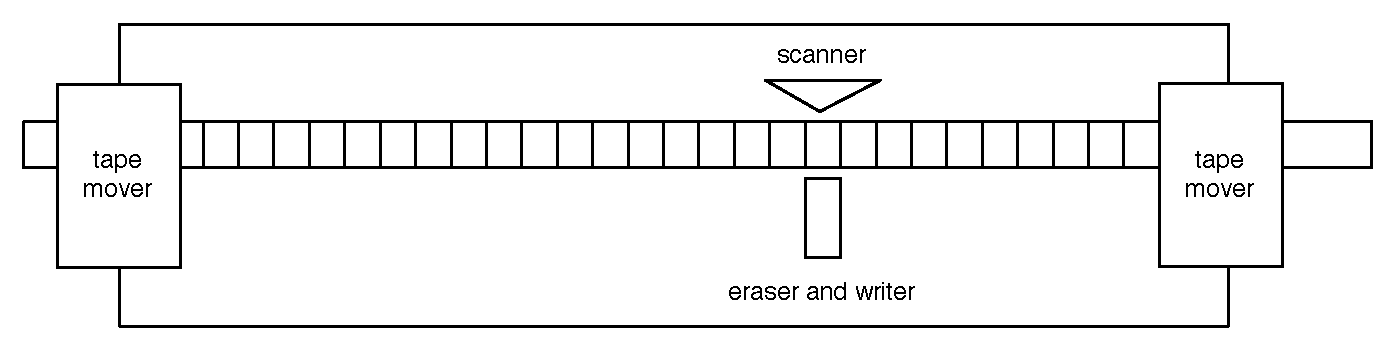
\includegraphics[width=0.9\textwidth]{turingmachine}
\caption{A Turing machine.}
\label{fig:machine}
\end{figure}


\begin{figure}
\centering
\subbottom[Turing Machine 1]{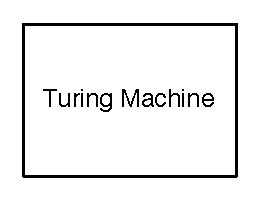
\includegraphics[width=0.2\textwidth]{block}\label{fig:tm:tm1}}
\subbottom[Turing Machine 2]{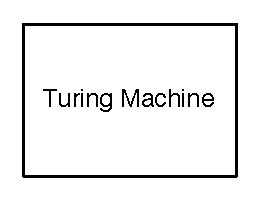
\includegraphics[width=0.2\textwidth]{block}\label{fig:tm:tm2}}
\subbottom[Turing Machine 3]{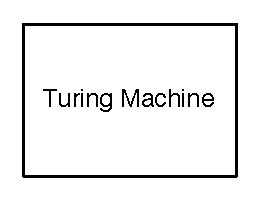
\includegraphics[width=0.2\textwidth]{block}\label{fig:tm:tm3}}
\subbottom[Turing Machine 4]{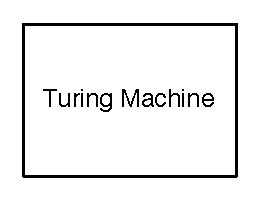
\includegraphics[width=0.2\textwidth]{block}\label{fig:tm:tm4}}
\caption{Plots of four Turing machines}
\label{fig:tm}
\end{figure}
